% A1 landscape poster (84.1 x 59.4 cm), four asymmetric quadrants:
%   top-left  : Muninn, what the paper does          | top-right    : our proposition
%   bottom-left: FM experiments -> the error found   | bottom-right : results (figures + table)
% Compile: latexmk -pdf poster.tex (or Overleaf, pdfLaTeX). Figures: python scripts/poster_figures.py
% Dashed grey boxes = figures still to produce (the box says what to run).
\documentclass[final]{beamer}
\usepackage[size=custom,width=84.1,height=59.4,scale=1.0]{beamerposter}
\usepackage[T1]{fontenc}
\usepackage[default]{lato}
\usepackage{amsmath,amssymb,bm}
\usepackage{graphicx,booktabs,tikz}
\usepackage[most]{tcolorbox}
\usetikzlibrary{positioning,arrows.meta,shapes.geometric,calc}

% ---------------------------------------------------------------- theme
\definecolor{ink}{HTML}{0B0B0B}
\definecolor{ink2}{HTML}{52514E}
\definecolor{blue}{HTML}{2A78D6}     % FewSteps AB2
\definecolor{orange}{HTML}{EB6834}   % our policy
\definecolor{aqua}{HTML}{1BAF7A}     % Muninn
\definecolor{paper}{HTML}{FCFCFB}
\definecolor{tintA}{HTML}{EEF4FC}    % Muninn quadrant
\definecolor{tintB}{HTML}{F3F2EE}    % FM experiment quadrant
\definecolor{tintC}{HTML}{FDF0EA}    % proposition quadrant
\definecolor{tintD}{HTML}{EDF8F3}    % results quadrant
\setbeamercolor{background canvas}{bg=paper}
\setbeamercolor{normal text}{fg=ink}
\setbeamertemplate{navigation symbols}{}
\setbeamertemplate{itemize items}{\color{ink2}\raisebox{0.15ex}{\scalebox{0.8}{$\blacksquare$}}}
\setbeamersize{text margin left=0cm, text margin right=0cm}
\setlength{\parskip}{0.3cm}

% a quadrant: #1 accent colour, #2 tint, #3 number, #4 title, #5 height
\newtcolorbox{panel}[5]{enhanced, colback=#2, colframe=#2, arc=10pt, boxrule=0pt,
  left=1.0cm, right=1.0cm, top=0.7cm, bottom=0.6cm, height=#5, valign=top, fontupper=\normalsize,
  before upper={{\LARGE\bfseries\color{#1}#3\hskip0.6cm#4}\par\vskip0.15cm{\color{#1}\rule{\linewidth}{4pt}}\par\vskip0.1cm}}
\newcommand{\sub}[2]{\vskip0.25cm{\large\bfseries\color{#1}#2}\par\vskip0.05cm}
% placeholder figure: #1 width, #2 height, #3 what it shows, #4 how to get it
\newcommand{\placeholder}[4]{%
  \tikz{\node[draw=ink2, dashed, line width=2pt, fill=white, rounded corners=8pt, minimum width=#1,
    minimum height=#2, text width=\dimexpr#1-1.4cm\relax, align=left, inner sep=0.6cm]
    {{\large\bfseries\color{orange} FIGURE TO PRODUCE}\\[0.2cm]\textbf{Shows:} #3\\[0.2cm]
     {\small\color{ink2}\textbf{Run:} #4}};}}

\newlength{\gap}\setlength{\gap}{1.2cm}
\newlength{\leftw}\setlength{\leftw}{0.40\paperwidth}
\newlength{\rightw}\setlength{\rightw}{\dimexpr\paperwidth-\leftw-3\gap\relax}
\newlength{\bodyh}\setlength{\bodyh}{49.4cm}
\newlength{\tlh}\setlength{\tlh}{16.2cm}   % top-left height (left split is higher than the right one)
\newlength{\trh}\setlength{\trh}{20.0cm}   % top-right height

\begin{document}
\begin{frame}[t]

% ---------------------------------------------------------------- header
\vskip0.6cm
\hskip\gap\begin{minipage}[c]{0.74\paperwidth}
  {\fontsize{62}{72}\selectfont\bfseries Certified step caching for flow-matching planners}\\[0.3cm]
  {\fontsize{36}{44}\selectfont\color{blue} Why Muninn's certificate fails, and what actually saves network calls}
\end{minipage}\hfill
\begin{minipage}[c]{0.2\paperwidth}\raggedleft
  {\Large\bfseries Author One, Author Two}\\[0.2cm]
  {\large\color{ink2} Affiliation\\ contact@email}
\end{minipage}\hskip\gap
\vskip0.5cm

\hskip\gap
% ================================================================ LEFT COLUMN
\begin{minipage}[t][\bodyh][t]{\leftw}\vspace{0pt}

% ---------------------------------------------------------------- 1. Muninn
\begin{panel}{aqua}{tintA}{1}{Muninn: caching with a certificate}{\tlh}
A diffusion / flow planner builds a plan by integrating $\dot x = v_\theta(x, t \mid c)$ over $N$ steps,
\textbf{one network call per step}. Muninn skips calls when the output barely changes:
\begin{itemize}
  \item \textbf{Probe}: run only the first block; change score $s_k = \lVert F_k - F_{\text{last}}\rVert_1 / \lVert F_{\text{last}}\rVert_1$.
  \item \textbf{Bound}: a conformal fit $U(s)$ predicts the reuse error $\lVert e_k\rVert$.
  \item \textbf{Budget}: reuse the last output while $\sum_k L_k\, U(s_k) \le \eta$, claiming
    $d(\text{fast plan}, \text{full plan}) \le \eta$.
\end{itemize}
\vskip0.3cm
\centering
\resizebox{0.94\linewidth}{!}{%
\begin{tikzpicture}[every node/.style={font=\Large}]
  \foreach \i/\r in {0/0,1/0,2/1,3/1,4/0,5/1,6/1,7/1,8/0,9/0} {
    \pgfmathsetmacro{\x}{\i*3.4}
    \ifnum\r=0
      \node[circle, fill=blue, minimum size=1.2cm, text=white] (n\i) at (\x,0) {\bfseries C};
    \else
      \node[circle, draw=aqua, line width=2.5pt, fill=white, minimum size=1.2cm, text=aqua] (n\i) at (\x,0) {\bfseries R};
    \fi
    \node[rectangle, draw=ink2, line width=1.2pt, minimum width=0.9cm, minimum height=0.5cm, fill=white] (p\i) at (\x,1.6) {};
    \draw[-{Stealth}, line width=1.5pt, ink2] (p\i) -- (n\i);
  }
  \foreach \i [evaluate=\i as \j using int(\i+1)] in {0,...,8} \draw[-{Stealth}, line width=2pt, ink2] (n\i) -- (n\j);
  \node[anchor=west] at (-0.8,2.7) {\color{ink2} probe at every step (cheap)};
  \node[anchor=west, text=blue] at (-0.8,-1.8) {\bfseries C = compute (1 call)};
  \node[anchor=east, text=aqua] at (31.4,-1.8) {\bfseries R = reuse last output (0 calls)};
\end{tikzpicture}}
\end{panel}

\vskip\gap
% ---------------------------------------------------------------- 2. FM experiments -> error
\begin{panel}{ink2}{tintB}{2}{On flow matching, the certificate breaks}{\dimexpr\bodyh-\tlh-\gap\relax}
\textbf{Motivation.} We port Muninn to flow matching (velocity reuse, Euler grid) on 2D toys and
compare it with \textbf{FewSteps}: simply fewer uniform steps.
\begin{itemize}
  \item At equal calls, FewSteps is \textbf{5--15$\times$ more accurate}, even against an oracle that
    knows the true reuse error.
  \item The certificate is \textbf{violated}: the oracle breaks $d \le \sum_k h\lVert e_k\rVert$ on
    \textbf{22--77\%} of samples.
\end{itemize}
\placeholder{\linewidth}{5.6cm}{per-sample actual deviation $d$ vs the paper's bound and vs our corrected bound
(above the diagonal = certificate violated), checkerboard toy.}{\texttt{python scripts/theory\_check.py --ckpt runs/toy\_checkerboard/model.pt},
then save panel 1 as \texttt{poster/figures/fig\_bound.pdf} (the per-sample points are not stored yet).}

\sub{ink2}{The missing term}
With $\Delta_k$ the gap to the full chain, the exact recursion is
\[
  \Delta_{k+1} = (I + h\bar J_k)\,\Delta_k + h\,e_k
  \;\Rightarrow\;
  \Delta_N = \sum_k h\, G_{k+1\to N}\, e_k, \quad G_{k+1\to N} = \prod_{j>k}(I + hJ_j).
\]
\begin{minipage}[t]{0.42\linewidth}\vspace{0pt}
The paper sets $G = I$. For flow matching (Tweedie)
\[
  \frac{\partial v}{\partial x} = \frac{1}{1-t}\Big[\frac{t\,\mathrm{Cov}(x_1 \mid x_t)}{(1-t)^2} - I\Big]
\]
so errors are \textbf{amplified where the final mode is still undecided} (up to $\times 900$).
\end{minipage}\hfill
\begin{minipage}[t]{0.56\linewidth}\vspace{0pt}
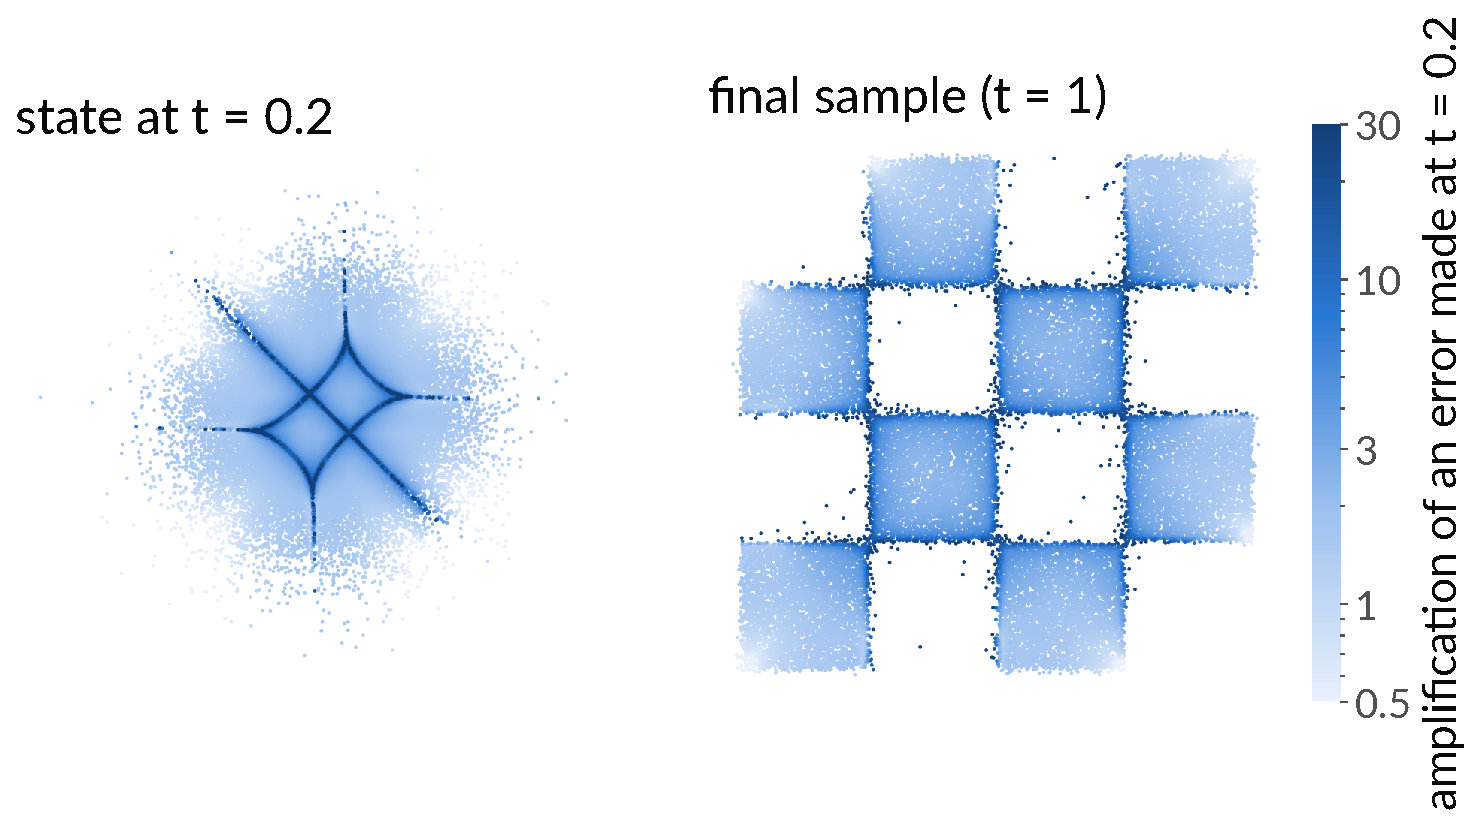
\includegraphics[width=\linewidth]{figures/fig_amplification.pdf}
\end{minipage}
\end{panel}

\end{minipage}%
\hskip\gap
% ================================================================ RIGHT COLUMN
\begin{minipage}[t][\bodyh][t]{\rightw}\vspace{0pt}

% ---------------------------------------------------------------- 3. proposition
\begin{panel}{orange}{tintC}{3}{Our proposition}{\trh}
\begin{minipage}[t]{0.5\linewidth}\vspace{0pt}
\sub{orange}{(a) Certify the final plan, not each step}
One knob per method (number of steps, or a threshold $\tau$), set on 4\,000 calibration plans
as the cheapest setting passing a Learn-then-Test test:
\[
  P\big(d(\text{plan}, \text{exact plan}) > \eta\big) \le \alpha \quad\text{with prob.}\ 1-\delta .
\]
Valid for any sampler, no Lipschitz assumption, same guarantee for every method; it also repairs Muninn.
\sub{orange}{(b) Spend calls where errors are amplified}
\begin{itemize}
  \item \textbf{Extrapolate} the velocity from the last two calls (instead of reusing it), on an \textbf{AB2} grid.
  \item Decide with the \textbf{amplified cost} $c_k = h\lVert G_{k+1\to N}\, e_k\rVert$.
  \item Predict $c_k$ from \textbf{free signals} (time, lag, recent rates of change), with a small
    regressor trained offline on exact targets. No probe.
\end{itemize}
\end{minipage}\hfill
\begin{minipage}[t]{0.46\linewidth}\vspace{0pt}
\vskip0.3cm
\centering
\resizebox{0.95\linewidth}{!}{%
\begin{tikzpicture}[node distance=0.9cm and 1.1cm, every node/.style={font=\Large},
  box/.style={draw=ink2, rounded corners=6pt, line width=1.5pt, align=center, inner sep=10pt, fill=white},
  arr/.style={-{Stealth[length=10pt]}, line width=2pt, color=ink2}]
  \node[box] (s) {free signals\\{\large time, lag, rates}};
  \node[box, right=of s] (p) {predicted\\ cost $\hat c_k$};
  \node[diamond, draw=ink2, line width=1.5pt, aspect=1.6, inner sep=1pt, minimum width=5cm, right=of p, fill=white] (d) {$\hat c_k \le \tau$?};
  \node[box, below=1.6cm of d, xshift=-3.6cm, draw=orange, text=orange] (e) {extrapolate\\{\large 0 calls}};
  \node[box, below=1.6cm of d, xshift=3.6cm, draw=blue, text=blue] (c) {compute\\{\large 1 call}};
  \draw[arr] (s) -- (p); \draw[arr] (p) -- (d);
  \draw[arr] (d.south) -- node[left, pos=0.45, xshift=-4pt] {yes} (e.north);
  \draw[arr] (d.south) -- node[right, pos=0.45, xshift=4pt] {no} (c.north);
\end{tikzpicture}}
\vskip0.6cm
\begin{tcolorbox}[colback=white, colframe=ink2, boxrule=1.2pt, arc=6pt, left=0.5cm, right=0.5cm,
  fontupper=\small\ttfamily, title={\normalsize\bfseries\sffamily sampling one plan}, colbacktitle=white, coltitle=ink2]
for k = 0 .. N-1:\\
\ \ if k < 2: compute\\
\ \ else:\ \ c = predictor(free\_signals)\\
\ \ \ \ \ \ \ \ extrapolate if c <= tau and lag < 10\\
\ \ \ \ \ \ \ \ otherwise compute\\
\ \ x += h * (1.5 u\_k - 0.5 u\_\{k-1\})\ \ \ \# AB2\\
cost = number of computes
\end{tcolorbox}
\end{minipage}
\end{panel}

\vskip\gap
% ---------------------------------------------------------------- 4. results
\begin{panel}{blue}{tintD}{4}{Results on a real planner: Maze2D U-maze}{\dimexpr\bodyh-\trh-\gap\relax}
\begin{minipage}[t]{0.25\linewidth}\vspace{0pt}
\placeholder{\linewidth}{8.0cm}{same start / goal: plans of full Euler-100, certified Muninn, AB2 and ours on the maze, with call counts.}{new script: sample each certified setting on 3--4 contexts, draw with \texttt{maze\_maps}.}
\end{minipage}\hfill
\begin{minipage}[t]{0.365\linewidth}\vspace{0pt}
\centering
{\large\bfseries Paper's Muninn vs FewSteps}\\[0.1cm]
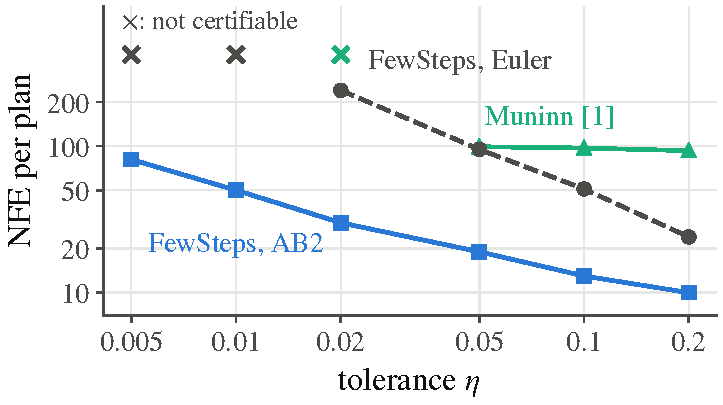
\includegraphics[width=\linewidth]{figures/fig_e18.pdf}
\end{minipage}\hfill
\begin{minipage}[t]{0.365\linewidth}\vspace{0pt}
\centering
{\large\bfseries Our policy vs FewSteps AB2}\\[0.1cm]
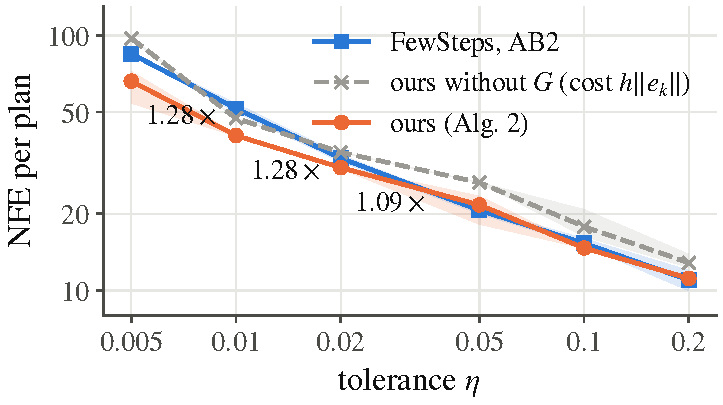
\includegraphics[width=\linewidth]{figures/fig_e19.pdf}
\end{minipage}

\vskip0.2cm
\begin{minipage}[t]{0.56\linewidth}\vspace{0pt}
\centering
\renewcommand{\arraystretch}{1.1}
\begin{tabular}{r rrrr r}
\toprule
 & \multicolumn{4}{c}{network calls per plan} & \\
\cmidrule(lr){2-5}
$\eta$ & Euler & Muninn & AB2 & \textbf{ours} & ours vs AB2 \\
\midrule
0.005 & -- & -- & 84.7 & \textbf{66.1} & \textbf{1.28$\times$} \\
0.01  & -- & -- & 51.7 & \textbf{40.5} & \textbf{1.28$\times$} \\
0.02  & 240 & -- & 33.0 & \textbf{30.3} & 1.09$\times$ \\
0.05  & 95 & 99 & \textbf{20.7} & 21.7 & 0.95$\times$ \\
0.1   & 51 & 97 & 15.3 & \textbf{14.7} & 1.04$\times$ \\
0.2   & 24 & 93 & \textbf{11.0} & 11.2 & 0.98$\times$ \\
\bottomrule
\end{tabular}\\[0.1cm]
{\small\color{ink2} $P(d > \eta) \le 5\%$ vs the exact ODE, 20\,000 test plans; -- = not certifiable; AB2, ours: 3 seeds.}
\end{minipage}\hfill
\begin{minipage}[t]{0.41\linewidth}\vspace{0pt}
\begin{itemize}
  \item Muninn skips only \textbf{1--7 of 100} calls: certified AB2 is \textbf{5--9$\times$} cheaper
    (2D toys: 6--14$\times$).
  \item Our policy: \textbf{1.28$\times$} fewer calls than AB2 at tight tolerances, ties at loose ones.
  \item Without $G$ it loses; Muninn's probe adds nothing.
\end{itemize}
\end{minipage}
\end{panel}

\end{minipage}
\end{frame}
\end{document}
